\documentclass[tikz,border=10pt]{standalone}
\usepackage{tikz}
\usetikzlibrary{arrows.meta,calc,positioning,shapes.geometric}

\tikzset{
  block/.style={draw=blue!70!black, line width=1.2pt, minimum width=2.2cm, minimum height=1.3cm, align=center},
  sum/.style={circle, draw=blue!70!black, line width=1.2pt, minimum size=8mm},
  sig/.style={-{Stealth[length=3mm]}, line width=1.2pt, draw=blue!70!black},
  note/.style={draw=orange!85!black, rounded corners=4pt, line width=1.1pt, minimum width=11.8cm, minimum height=0.95cm, align=center, text width=11.1cm}
}

\begin{document}
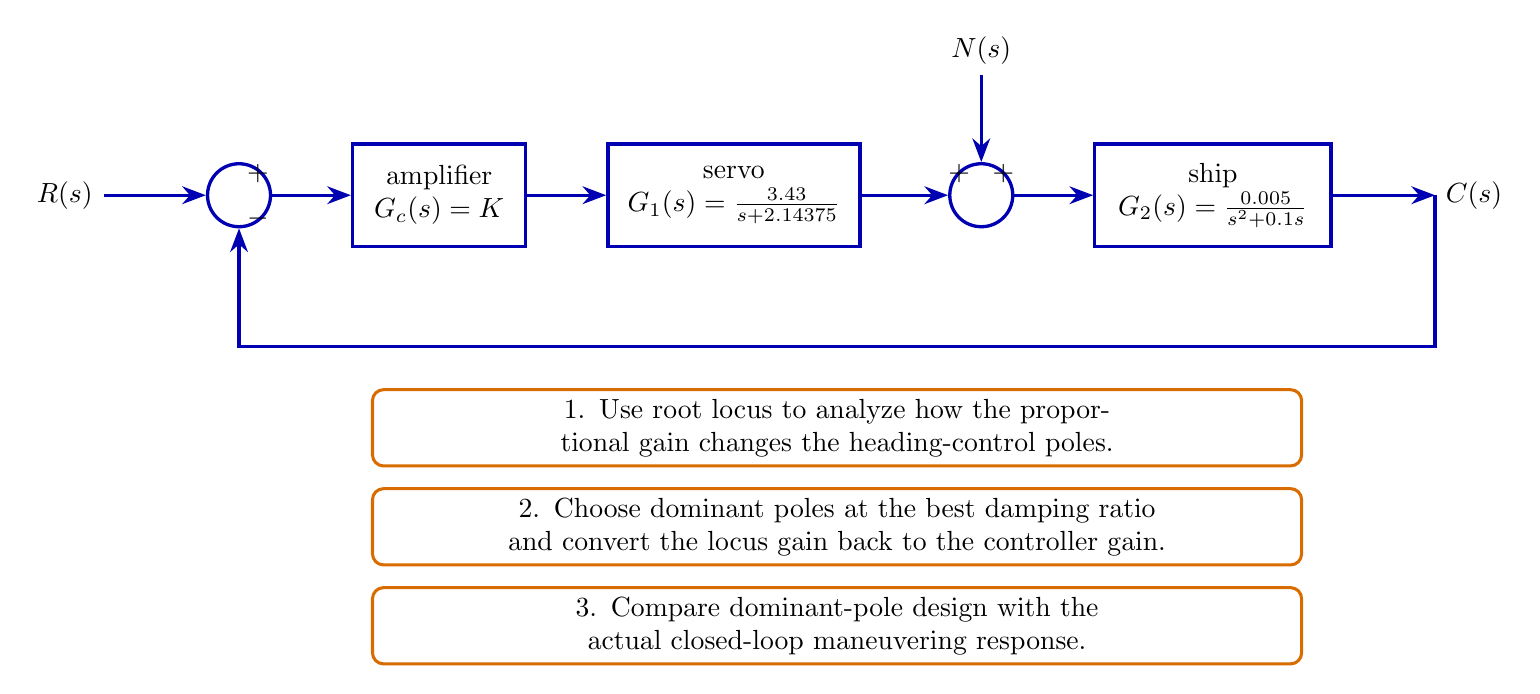
\begin{tikzpicture}[node distance=1.0cm]
  \node[sum] (s1) {};
  \node[block, right=1.0cm of s1] (gc) {amplifier\\$G_c(s)=K$};
  \node[block, right=1.0cm of gc, minimum width=3.2cm] (g1) {servo\\$G_1(s)=\frac{3.43}{s+2.14375}$};
  \node[sum, right=1.1cm of g1] (s2) {};
  \node[block, right=1.0cm of s2, minimum width=3.0cm] (g2) {ship\\$G_2(s)=\frac{0.005}{s^2+0.1s}$};
  \coordinate[right=1.3cm of g2] (out);

  \draw[sig] ($(s1.west)+(-1.3,0)$) node[left] {$R(s)$} -- (s1);
  \draw[sig] (s1) -- (gc);
  \draw[sig] (gc) -- (g1);
  \draw[sig] (g1) -- (s2);
  \draw[sig] (s2) -- (g2);
  \draw[sig] (g2) -- (out) node[right] {$C(s)$};
  \draw[sig] ($(s2.north)+(0,1.1)$) node[above] {$N(s)$} -- (s2);
  \draw[sig] (out) |- ($(s1.south)+(0,-1.5)$) -| (s1);

  \node at ($(s1)+(0.24,0.28)$) {$+$};
  \node at ($(s1)+(0.24,-0.30)$) {$-$};
  \node at ($(s2)+(-0.28,0.28)$) {$+$};
  \node at ($(s2)+(0.28,0.28)$) {$+$};

  \node[note, below=2.45cm of $(s1)!0.5!(out)$] (n1) {1. Use root locus to analyze how the proportional gain changes the heading-control poles.};
  \node[note, below=0.25cm of n1] (n2) {2. Choose dominant poles at the best damping ratio and convert the locus gain back to the controller gain.};
  \node[note, below=0.25cm of n2] (n3) {3. Compare dominant-pole design with the actual closed-loop maneuvering response.};
\end{tikzpicture}
\end{document}
